\documentclass[letterpaper,9pt,twocolumn,twoside,]{pinp}

%% Some pieces required from the pandoc template
\providecommand{\tightlist}{%
  \setlength{\itemsep}{0pt}\setlength{\parskip}{0pt}}

% Use the lineno option to display guide line numbers if required.
% Note that the use of elements such as single-column equations
% may affect the guide line number alignment.

\usepackage[T1]{fontenc}
\usepackage[utf8]{inputenc}

% pinp change: the geometry package layout settings need to be set here, not in pinp.cls
\geometry{layoutsize={0.95588\paperwidth,0.98864\paperheight},%
  layouthoffset=0.02206\paperwidth, layoutvoffset=0.00568\paperheight}

\definecolor{pinpblue}{HTML}{185FAF}  % imagecolorpicker on blue for new R logo
\definecolor{pnasbluetext}{RGB}{101,0,0} %



\title{Data analysis report - Root Insurance}

\author[a]{Issac Lee}

  \affil[a]{Department of Statistics \& Actuarial Science, 241 Schaeffer Hall, Iowa
City, Iowa 52242-1409}

\setcounter{secnumdepth}{0}

% Please give the surname of the lead author for the running footer
\leadauthor{Author and Author}

% Keywords are not mandatory, but authors are strongly encouraged to provide them. If provided, please include two to five keywords, separated by the pipe symbol, e.g:
 

\begin{abstract}
This report illustrates how I approach the project and the decision
making the process for Root insurance's data analysis project. The goal
of this project is to find the best-matched OBDII trip data, which
corresponds to a trip data from a user's smartphone. The data analysis
process appears in the first chapter, and the instructional manual
follows in the later chapter. The \texttt{R} code implementations follow
Google's \texttt{R} code style guide.
\end{abstract}

\dates{This version was compiled on \today} 

% initially we use doi so keep for backwards compatibility
% new name is doi_footer
\doifooter{\url{https://cran.r-project.org/package=YourPackage}}

\pinpfootercontents{YourPackage Vignette}

\begin{document}

% Optional adjustment to line up main text (after abstract) of first page with line numbers, when using both lineno and twocolumn options.
% You should only change this length when you've finalised the article contents.
\verticaladjustment{-2pt}

\maketitle
\thispagestyle{firststyle}
\ifthenelse{\boolean{shortarticle}}{\ifthenelse{\boolean{singlecolumn}}{\abscontentformatted}{\abscontent}}{}

% If your first paragraph (i.e. with the \dropcap) contains a list environment (quote, quotation, theorem, definition, enumerate, itemize...), the line after the list may have some extra indentation. If this is the case, add \parshape=0 to the end of the list environment.


\hypertarget{data-preparation}{%
\subsection{Data Preparation}\label{data-preparation}}

There are two telematics data set from independent sensors: GPS in
smartphone, OBDII. The two data sets are provided as two separate file.
Here we assume that the two \texttt{json} files are extracted in the
working directory, which means you have the following two files in the
working directory:

\begin{quote}
mobile\_trips.json, obd2\_trips.json
\end{quote}

\hypertarget{data-load-and-structure}{%
\subsection{Data load and structure}\label{data-load-and-structure}}

Since the two files are recorded as \texttt{json} format,
\texttt{jsonlite} package will be used to load the data.

\begin{Shaded}
\begin{Highlighting}[]
\KeywordTok{library}\NormalTok{(jsonlite)}

\CommentTok{# read mobile trip & obd2 trip}
\NormalTok{mobile_data <-}\StringTok{ }\KeywordTok{fromJSON}\NormalTok{(}\StringTok{"./mobile_trips.json"}\NormalTok{)}
\NormalTok{obd2_data <-}\StringTok{ }\KeywordTok{fromJSON}\NormalTok{(}\StringTok{"./obd2_trips.json"}\NormalTok{)}
\end{Highlighting}
\end{Shaded}

Smartphone data set consisists of 44 trips and OBDII data set consists
of 41 trips. The colum names of the each data set and the data types are
as follows:

\begin{itemize}
\tightlist
\item
  OBDII data

  \begin{itemize}
  \tightlist
  \item
    trip\_id (\texttt{char}), timestamp (\texttt{dbl}), speed
    (\texttt{int})
  \end{itemize}
\item
  Mobile data

  \begin{itemize}
  \tightlist
  \item
    trip\_id (\texttt{char}), created\_at (\texttt{dbl}), timestamp
    (\texttt{dbl}), speed (\texttt{dbl}), accuracy (\texttt{int})
  \end{itemize}
\end{itemize}

\hypertarget{visualization-of-sample-trips}{%
\subsection{Visualization of sample
trips}\label{visualization-of-sample-trips}}

Fig \ref{fig:rawplot_obd2} shows the speed graph of a sample trip from
OBDII data. As we can see, the OBDII trip was recorded for about 1,200
seconds and we do not know the unit for the recorded speed. Fig
\ref{fig:rawplot_mobile} shows the speed graph of a sample trip from
mobile data. Note that the scale of x-axis has been adjusted as zero. By
examing the data set littel bit, it can be easily realized that the
first trip from each sources corresponds to each other as in Fig.
\ref{fig:rawplot_obd2} and Fig \ref{fig:rawplot_mobile}. As we can see
the whole trip data from smartphone corresponds to the trip data from
OBDII around 300 seconds.

\begin{figure}

{\centering 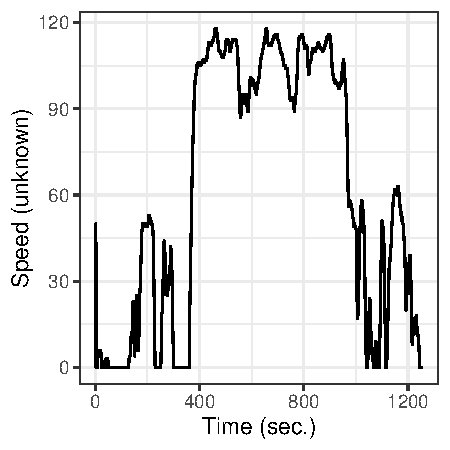
\includegraphics{report_issaclee_files/figure-latex/rawplot_obd2-1} 

}

\caption{A sample of speed graph of OBDII (the 1st trip).}\label{fig:rawplot_obd2}
\end{figure}

\begin{figure}

{\centering 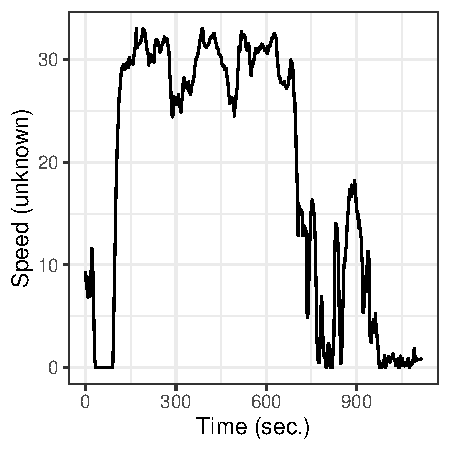
\includegraphics{report_issaclee_files/figure-latex/rawplot_mobile-1} 

}

\caption{A sample of speed graph of Smartphone (the 1st trip).}\label{fig:rawplot_mobile}
\end{figure}

\hypertarget{determine-the-conversion-factor-between-speed-scale}{%
\subsubsection{Determine the conversion factor between speed
scale}\label{determine-the-conversion-factor-between-speed-scale}}

Using this knowledge we found, we can figure out there is a conversion
factor between the two different speed scale from each sources. If
thoese sensor recorded the same trip, thier maximum speed should be the
same. Thus, we can calculate the conversion factor as follows:

\begin{Shaded}
\begin{Highlighting}[]
\CommentTok{# Conversion factor}
\KeywordTok{max}\NormalTok{(obd2_trip_sample1}\OperatorTok{$}\NormalTok{speed) }\OperatorTok{/}\StringTok{ }
\StringTok{  }\KeywordTok{max}\NormalTok{(mobile_trip_sample1}\OperatorTok{$}\NormalTok{speed)}
\end{Highlighting}
\end{Shaded}

\begin{ShadedResult}
\begin{verbatim}
#  [1] 3.570348
\end{verbatim}
\end{ShadedResult}

We can see that it is around 3.6. There are many units for speed such as
miles per hour (mph), kilometers per hour (km/h), etc. Using the cue
that the smartphone sensor should use either \texttt{mph} or
\texttt{km/h}, we can easily guess that the OBDII uses \texttt{m/s}
since the relationship between \texttt{km/h} and \texttt{m/s} is as
follows:

\[
1 \ m/s = 3.6 \ km/h
\]

Thus, using conversion factor and the lagging time (300 sec.), we can
guess our final output should be similar to Fig \ref{fig:speedplot}.
From now on, we will use \texttt{km/h} as a speed scale since the result
plot re-confirms that the unit of each sensors.

\begin{figure}

{\centering 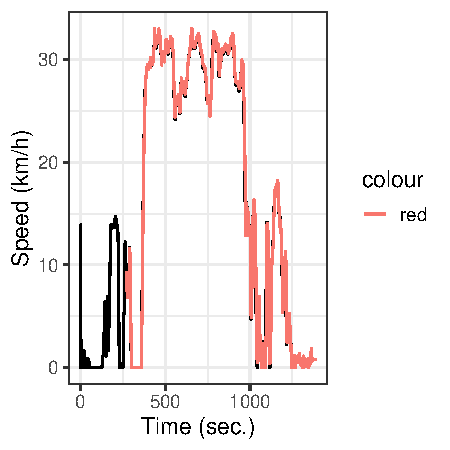
\includegraphics{report_issaclee_files/figure-latex/speedplot-1} 

}

\caption{A sample output of matched speed graph.}\label{fig:speedplot}
\end{figure}

\hypertarget{lagging-time-detection-algorithm}{%
\subsection{Lagging time detection
algorithm}\label{lagging-time-detection-algorithm}}

The next step is to automatically determine the lag time given that we
have two matched trips. We will use the same sample trips used in the
previous section. In Fig. \ref{fig:speedplot}, the exact lag time for
smartphone trip data was 270 seconds. To detect the lagging time, we
need to consider every possible combination of these two trip by using
sliding window algorithm. A nice visualization of this concept can be
found at
\href{https://en.wikipedia.org/wiki/Convolution\#/media/File:Convolution_of_spiky_function_with_box2.gif}{here}.
We consider the speed graph from OBDII as a fixed function and the speed
graph from smartphone as a floating function in the algorithm.

Let \(x \in \mathbb{R^+}\) be a real positive vector of size \(n_x\)
whose elements represent the speeds or a trip from smartphone, while
\(y \in \mathbb{R^+}\) and \(n_y\) represents the speed and the size of
the speed vector from OBDII repectively.

\begin{equation*}
  \begin{aligned}
    x & = (x_1, x_2, ..., x_{n_x})^T \\
    y & = (y_1, y_2, ..., y_{n_y})^T
  \label{eqn:speedvector} 
  \end{aligned}
\end{equation*}

To implement the sliding window algorithm, we uses a dummy variable
\texttt{k} from 1 to \(n_x + n_y\) to search all the possible overlapped
combination of the two graph. For example, when \(k = 1\), we consider
the situation where \(x_{n_x}\) and \(y_1\) are overlapped each other.
When \(k=2\), \((x_{n_x - 1}, x_{n_x})\) and \((y_1, y_2)\) are
considered. Thus, for any \(k \leq n_x+n_y\) where \(k \in \mathbb{N}\),
the overlapped vectors, \(x^*\) and \(y^*\) can be written as follows;

\begin{equation}
  \begin{aligned}
  x^* &= (max(n_x - k, 1), ..., n_x - max(0, k - n_y))^T \\
  y^* &= (max(k-n_x, 1), ..., min(n_y, k))^T
  \label{eqn:slidingwindow} 
  \end{aligned}
\end{equation}

Equation \ref{eqn:slidingwindow} shows the compact expression for the
three cases:

\begin{itemize}
\tightlist
\item
  Case 1: \(k < n_x\) and \(k < n_y\)

  \begin{itemize}
  \tightlist
  \item
    \(x^* = (n_x - k, ..., n_x)\)
  \item
    \(y^* = (1, ..., k)\)
  \end{itemize}
\item
  Case 2: \(k > n_x\) and \(k < n_y\)

  \begin{itemize}
  \tightlist
  \item
    \(x^* = (1, ..., n_x)\)
  \item
    \(y^* = (k-n_x, ..., k)\)
  \end{itemize}
\item
  Case 3: \(k > n_x\) and \(k > n_y\)

  \begin{itemize}
  \tightlist
  \item
    \(x^* = (1, ..., n_y - (k-n_x))\)
  \item
    \(y^* = ((k-n_x), ..., n_y)\)
  \end{itemize}
\end{itemize}

\hypertarget{measure-for-the-similarity}{%
\subsection{Measure for the
similarity}\label{measure-for-the-similarity}}

There are many measures for the similarity of the two functions whose
domains are the same: area under the difference of the two functions,
maximum difference of the two functions values, etc. Among these, the
following measure is used for detecting the similarity between the two
speed vectors:

\begin{equation}
  \begin{aligned}
 f(x, y) = \frac{\sqrt{\left(\sum_{i\in A}\left(x_{i}-y_{i}\right)^{2}\right)}}{|A|} + \frac{\lambda}{|A|}
  \label{eqn:sumofsquare} 
  \end{aligned}
\end{equation} where the vector \(x\) and \(y\) are the speed vector
from smartphone and OBDII, and the set \(A\) is the collection of the
pair of coordinates of OBDII and smartphone speed vectors overlapped
each other for fixed \(k\). Note that the function \(|.|\) indicates the
caldinality of a set. The reason of the division in Equation
\ref{eqn:sumofsquare} is to calculate the average of the errors.

Also, the second term can be thought as a penalty function that prevents
the case where the length of the overlapped is too short, so the
dissimilarity is too small. We can put the weights on the panalty using
\(\lambda\), and we uses 10 for \(\lambda\) value for this case. Since
the value of \(f(x, y)\) decreases when the two vector \(x\) and \(y\)
are similar to each other, the interpretation of the measure should be
dissimilarity of the two vector. Fig. \ref{fig:laggedtime} shows the
dissimilarity with respect to the \(k\) from 1 to 2354, which is the
summation of the length of speed vector from OBDII and smartphone. The
index which makes the dissimilarity to be the smallest value is
\(k = 1374\). According to Equation \ref{eqn:slidingwindow}, this
corresponds to the 255th time stamp of the OBDII trip.

\begin{figure}

{\centering 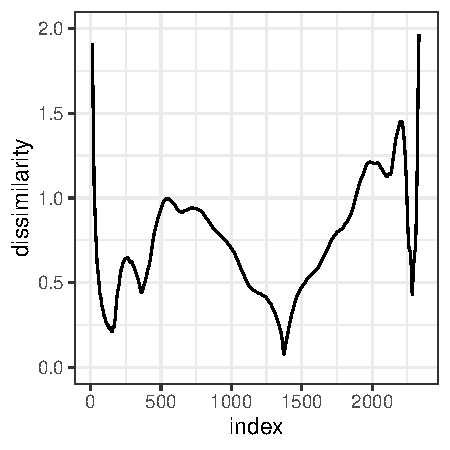
\includegraphics{report_issaclee_files/figure-latex/laggedtime-1} 

}

\caption{Dissimilarity measure for w.r.t. $k$}\label{fig:laggedtime}
\end{figure}

\hypertarget{find-the-best-matched-trips}{%
\subsection{Find the best matched
trips}\label{find-the-best-matched-trips}}

In the previous section, we have discussed how to find the lagging time
using dissimilarity measure. To find a best matched trip among the
collection of the OBDII trips for a given smartphone trip, we can find
the OBDII trip whose minimum of the dissmilarity with the given
smartphone trip is the lowest among the whole collection of the OBDII
data set. However, since we cannnot guarantee that the lowest minimum of
the dissmilarity implies that the two trip from each sources actually
matched each other, we set \(0.1\) as a threshold. Thus, if the lowest
minimum dissimilarity is less than 0.1, we decide that the pair of OBDII
trip and smartphone trip are matched each other. Fig.
\ref{fig:dissimilarity} represents the minimum of dissimilarity for each
trips in OBDII data with the first trip in mobile data set. The dotted
line, in Fig. \ref{fig:dissimilarity}, indicates the threshold for
matched trip. Since the minimum of the dissimilarity of the first trip
is less than the 0.1, we choose the first trip in OBDII data as the best
matched trip with the first trip in mobile data.

\begin{figure}

{\centering 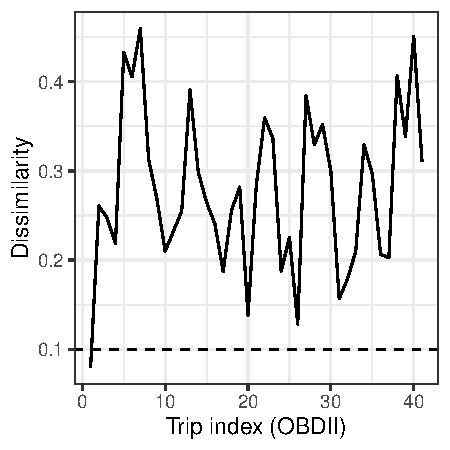
\includegraphics{report_issaclee_files/figure-latex/dissimilarity-1} 

}

\caption{Minimum values of dissimilarity for each trips in OBDII data set}\label{fig:dissimilarity}
\end{figure}

\hypertarget{user-instruction}{%
\subsection{User instruction}\label{user-instruction}}

\hypertarget{load-data}{%
\subsubsection{Load data}\label{load-data}}

You can load the JSON file into \texttt{R} using \texttt{jsonlite}
package as at the biginning of this document.

\begin{Shaded}
\begin{Highlighting}[]
\KeywordTok{library}\NormalTok{(jsonlite)}

\CommentTok{# read mobile trip & obd2 trip}
\NormalTok{mobile_data <-}\StringTok{ }\KeywordTok{fromJSON}\NormalTok{(}\StringTok{"./mobile_trips.json"}\NormalTok{)}
\NormalTok{obd2_data <-}\StringTok{ }\KeywordTok{fromJSON}\NormalTok{(}\StringTok{"./obd2_trips.json"}\NormalTok{)}
\end{Highlighting}
\end{Shaded}

\hypertarget{find-the-best-obdii-trip-for-given-smartphone-trip}{%
\subsubsection{Find the best OBDII trip for given smartphone
trip}\label{find-the-best-obdii-trip-for-given-smartphone-trip}}

The following code will find the best OBDII trip which matches with
\texttt{given\_trip} mobile trip, and save the information into
\texttt{match\_info}.

\begin{Shaded}
\begin{Highlighting}[]
\CommentTok{# Select the second trip in the mobile data set}
\NormalTok{given_trip <-}\StringTok{ }\NormalTok{mobile_data[[}\DecValTok{2}\NormalTok{]]}

\CommentTok{# Find the best trip from OBDII data set}
\NormalTok{match_info <-}\StringTok{ }\KeywordTok{FindBestTrip}\NormalTok{(given_trip, obd2_data)}
\end{Highlighting}
\end{Shaded}

The \texttt{match\_info} variable has the matched result information. We
can see that there are seven information as follows:

\begin{Shaded}
\begin{Highlighting}[]
\KeywordTok{summary}\NormalTok{(match_info)}
\end{Highlighting}
\end{Shaded}

\begin{ShadedResult}
\begin{verbatim}
#                  Length Class  Mode   
#  start_index_ref 1      -none- numeric
#  start_index_tar 1      -none- numeric
#  overlap_length  1      -none- numeric
#  dissimilarity   1      -none- numeric
#  macthed_trip    1      -none- numeric
\end{verbatim}
\end{ShadedResult}

\begin{Shaded}
\begin{Highlighting}[]
\CommentTok{# Visualization}
\KeywordTok{VisTrip}\NormalTok{(given_trip, obd2_data, match_info)}
\end{Highlighting}
\end{Shaded}

\begin{center}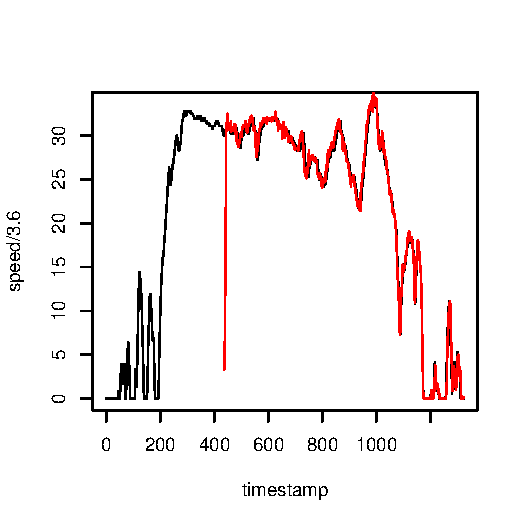
\includegraphics{report_issaclee_files/figure-latex/unnamed-chunk-7-1} \end{center}

%\showmatmethods


\bibliography{pinp.bib}
\bibliographystyle{jss}



\end{document}

